\documentclass[12pt,a4paper,oneside]{article}
\usepackage[colorlinks=true, unicode]{hyperref}
\usepackage[utf8]{inputenc}
\usepackage[czech]{babel}
\usepackage{graphicx}
\usepackage{pdfpages}
\textwidth 16cm \textheight 25cm
\topmargin -1.3cm 
\oddsidemargin 0cm
\usepackage{footnote}
\pagestyle{empty}
\begin{document}
\title{Rychlý USB 2.0 komunikační modul USBIO01A}
\author{Jakub Kákona, kaklik@mlab.cz}
\maketitle

\thispagestyle{empty}
\begin{abstract}
Modul umožňuje řízení digitálních výstupů přes USB a také rychlý přenos paralelních dat. Je založen na čipu CY7C68013A. Podporuje high-speed komunikaci USB 2.0.
\end{abstract}

\begin{figure} [htbp]
\begin{center}
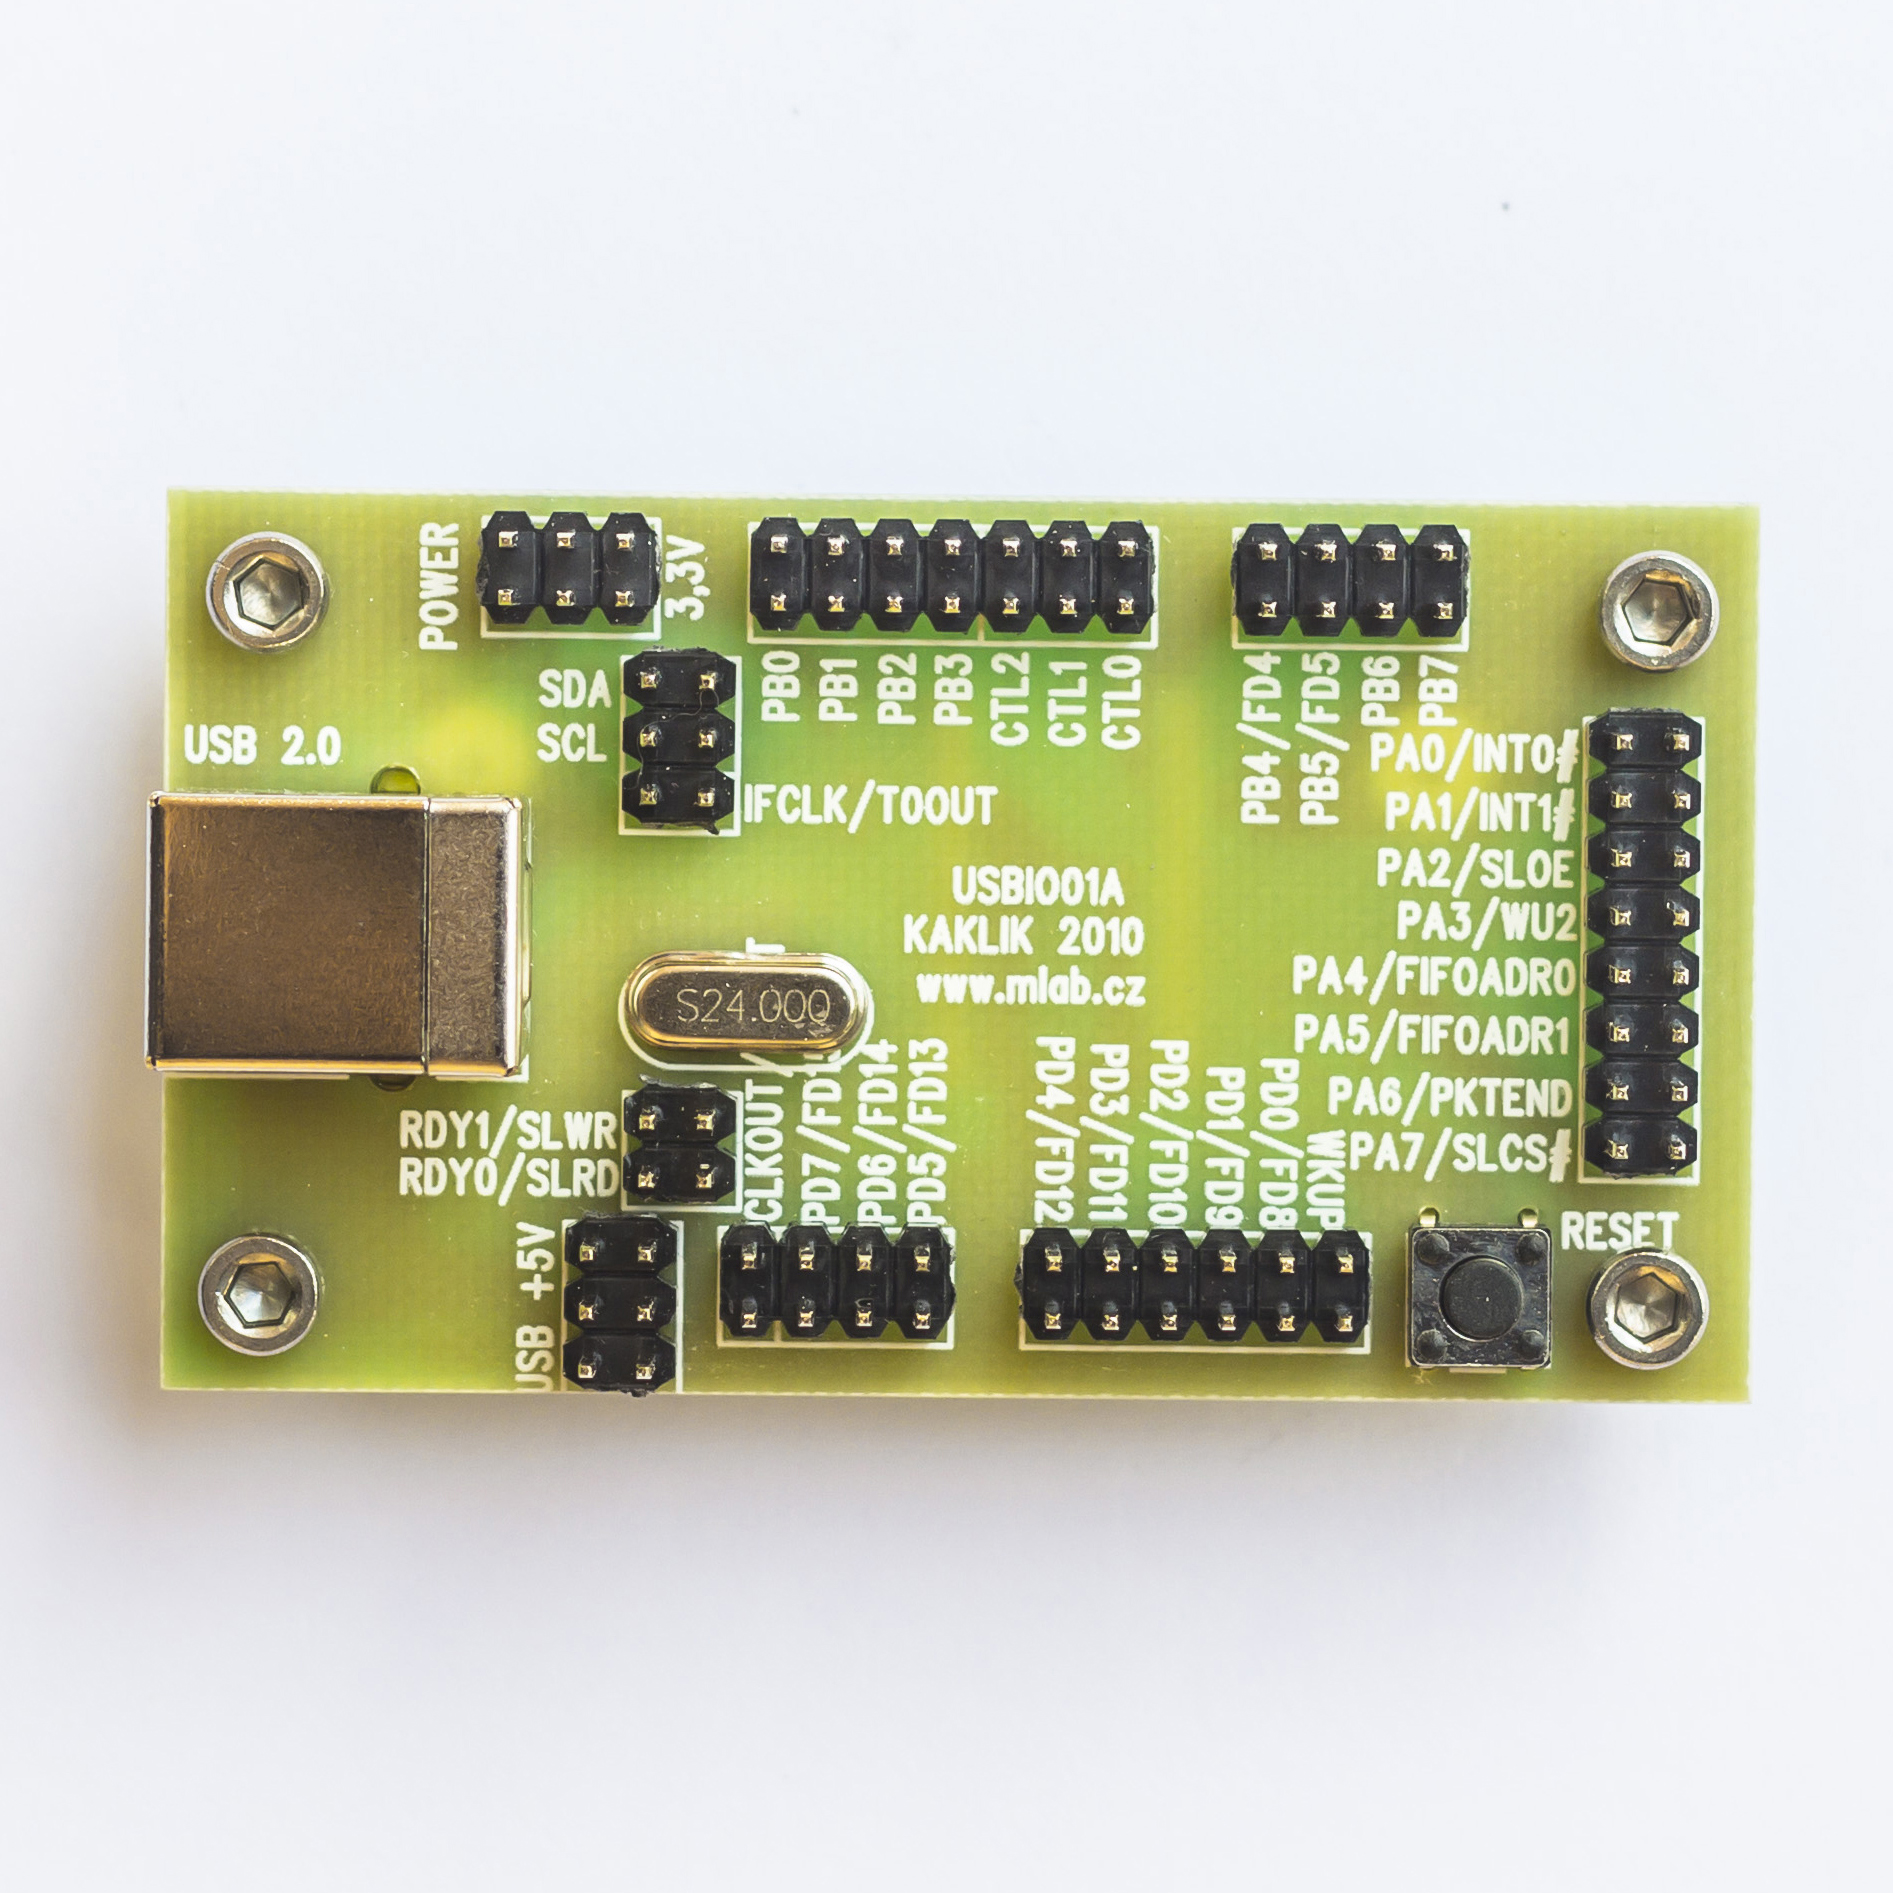
\includegraphics [width=100mm] {./img/USBIO01A_Top_Big.jpg} 
\end{center}
\end{figure}

\begin{figure} [b]

\includegraphics [width=25mm] {./img/USBIO01A_QRcode.png} 
\end{figure}

\newpage
\tableofcontents

\section{Technické parametry}
\begin{table}[htbp]
\begin{center}
\begin{tabular}{|c|c|p{4.7cm}|}
\hline
Parametr & Hodnota & Poznámka \\
\hline
Napájecí napětí & USB +5V &  USB napájení je vyvedeno i jako výstup \\ 
\hline
\end{tabular}
\end{center}
\end{table}

\section{Popis konstrukce}

\subsection{Zapojení}

Modul obsahuje minimální množství součástek potřebné pro funkci čipu CY7C68013A. Tento čip má 3.3V logické výstupy, které jsou 5V tolerantní. Napájecí napětí 3.3V je stabilizováno lineárním stabilizátorem, který je součástí zapojení plošného spoje. Korektní napěťový reset obvodu CY7C68013A je vyřešen resetovacím obvodem TCM809. 

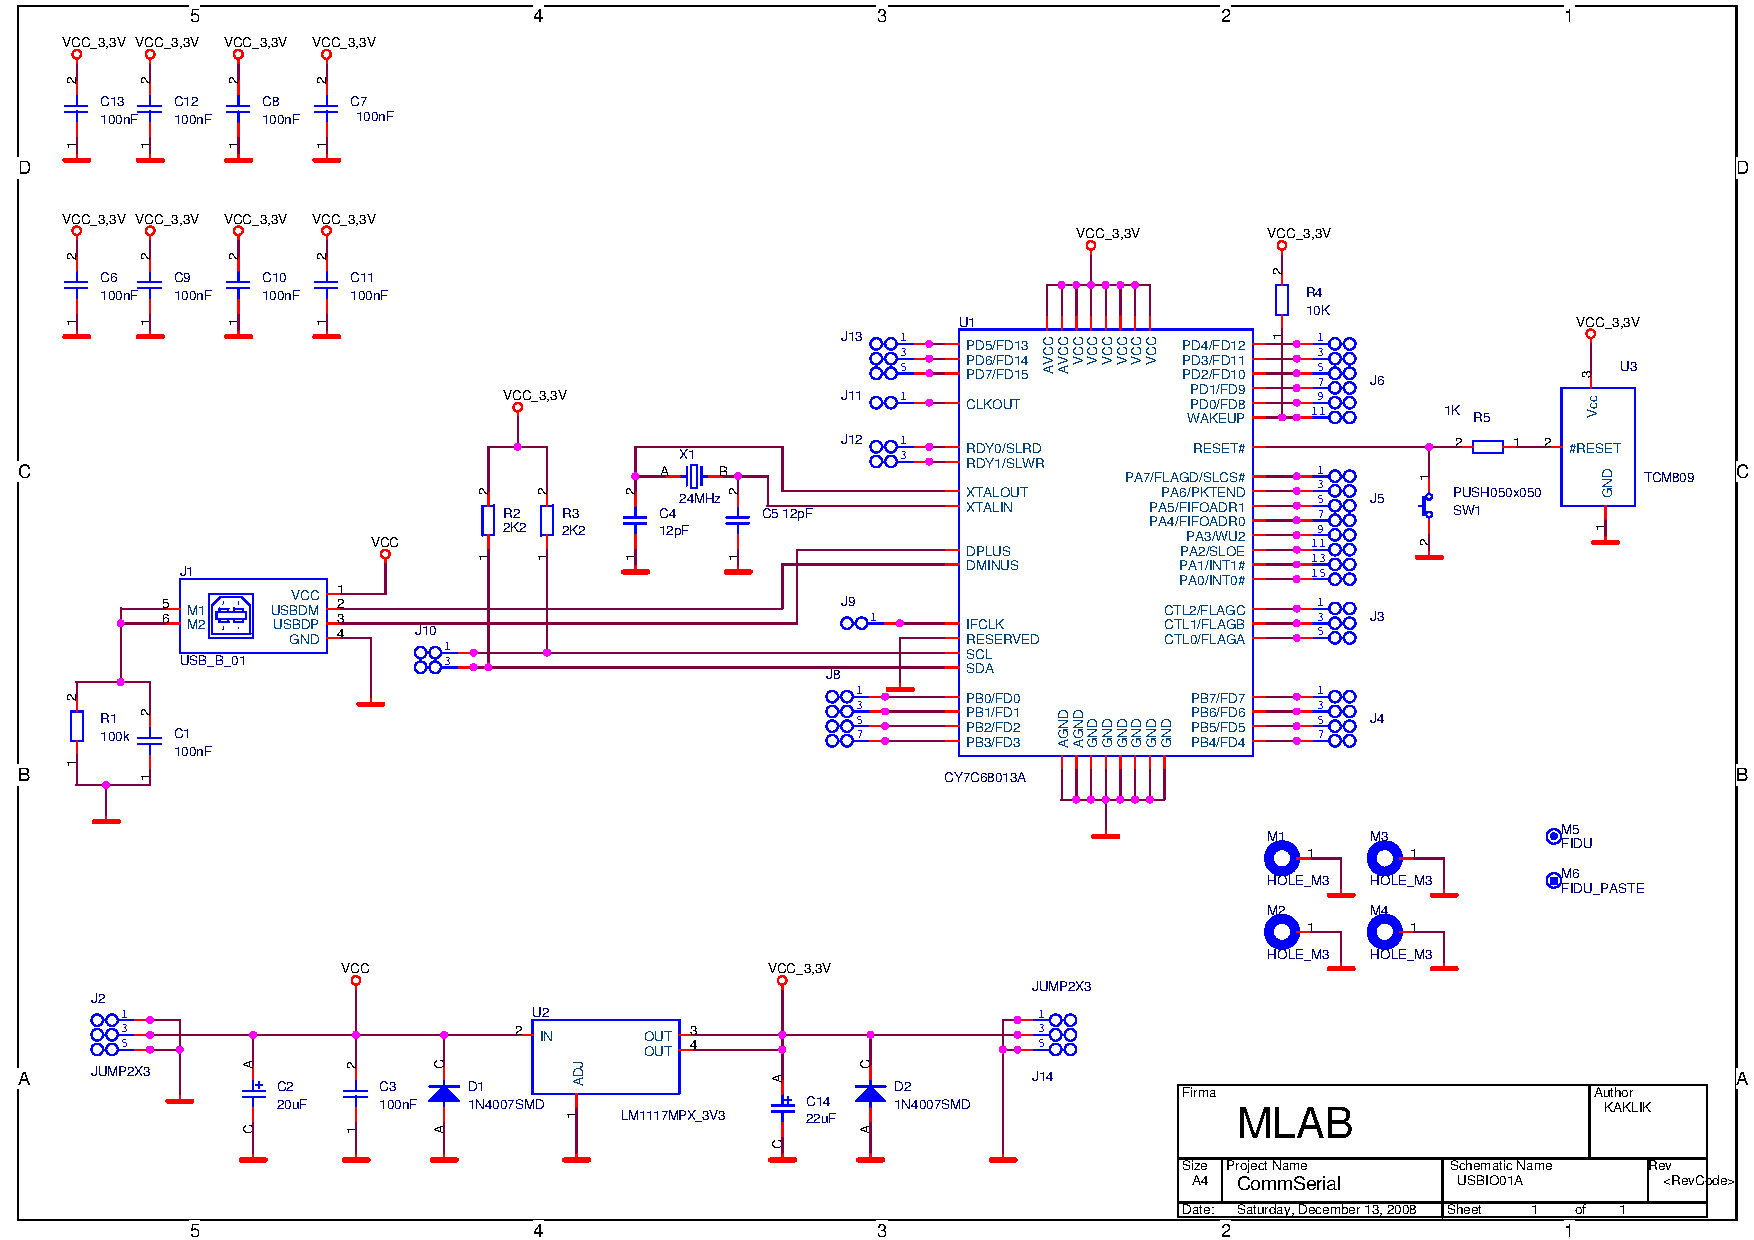
\includepdf[pages={1},landscape=true]{../../SCH/USBIO.pdf}

Pro trvalé nahrání firmware zařízení založeného na tomto USB mikrokontroleru se předpokládá připojení externí I$^2$C EEPROM do které je nahrán firmware. Tato EEPROM není součástí zapojení modulu a je v takovém případě potřebné využít další modul.


\subsection{Mechanická konstrukce}

Modul klasicky předpokládá uchycení na čtyřech šroubech, které by pro správnou funkci modulu měly být spojeny s vodivou zemí.  

\section{Výroba a testování}

Plošný spoj je navržen jak pro ruční pájení, tak i pro osazování pomocí pasty.  Modul se testuje optickou kontrolou spojů a následným připojením na laboratorní zdroj s omezením proudu. Dále by po připojení mikrokontroleru na USB mělo dojít k enumeraci USB zařízení. 

\subsubsection{Osazení}

Modul je možné osadit i ručně. Rozložení součástek je na Obr. \ref{fig:osazovaci_plan}. 

\begin{figure} [h!tbp]
  \centering
  %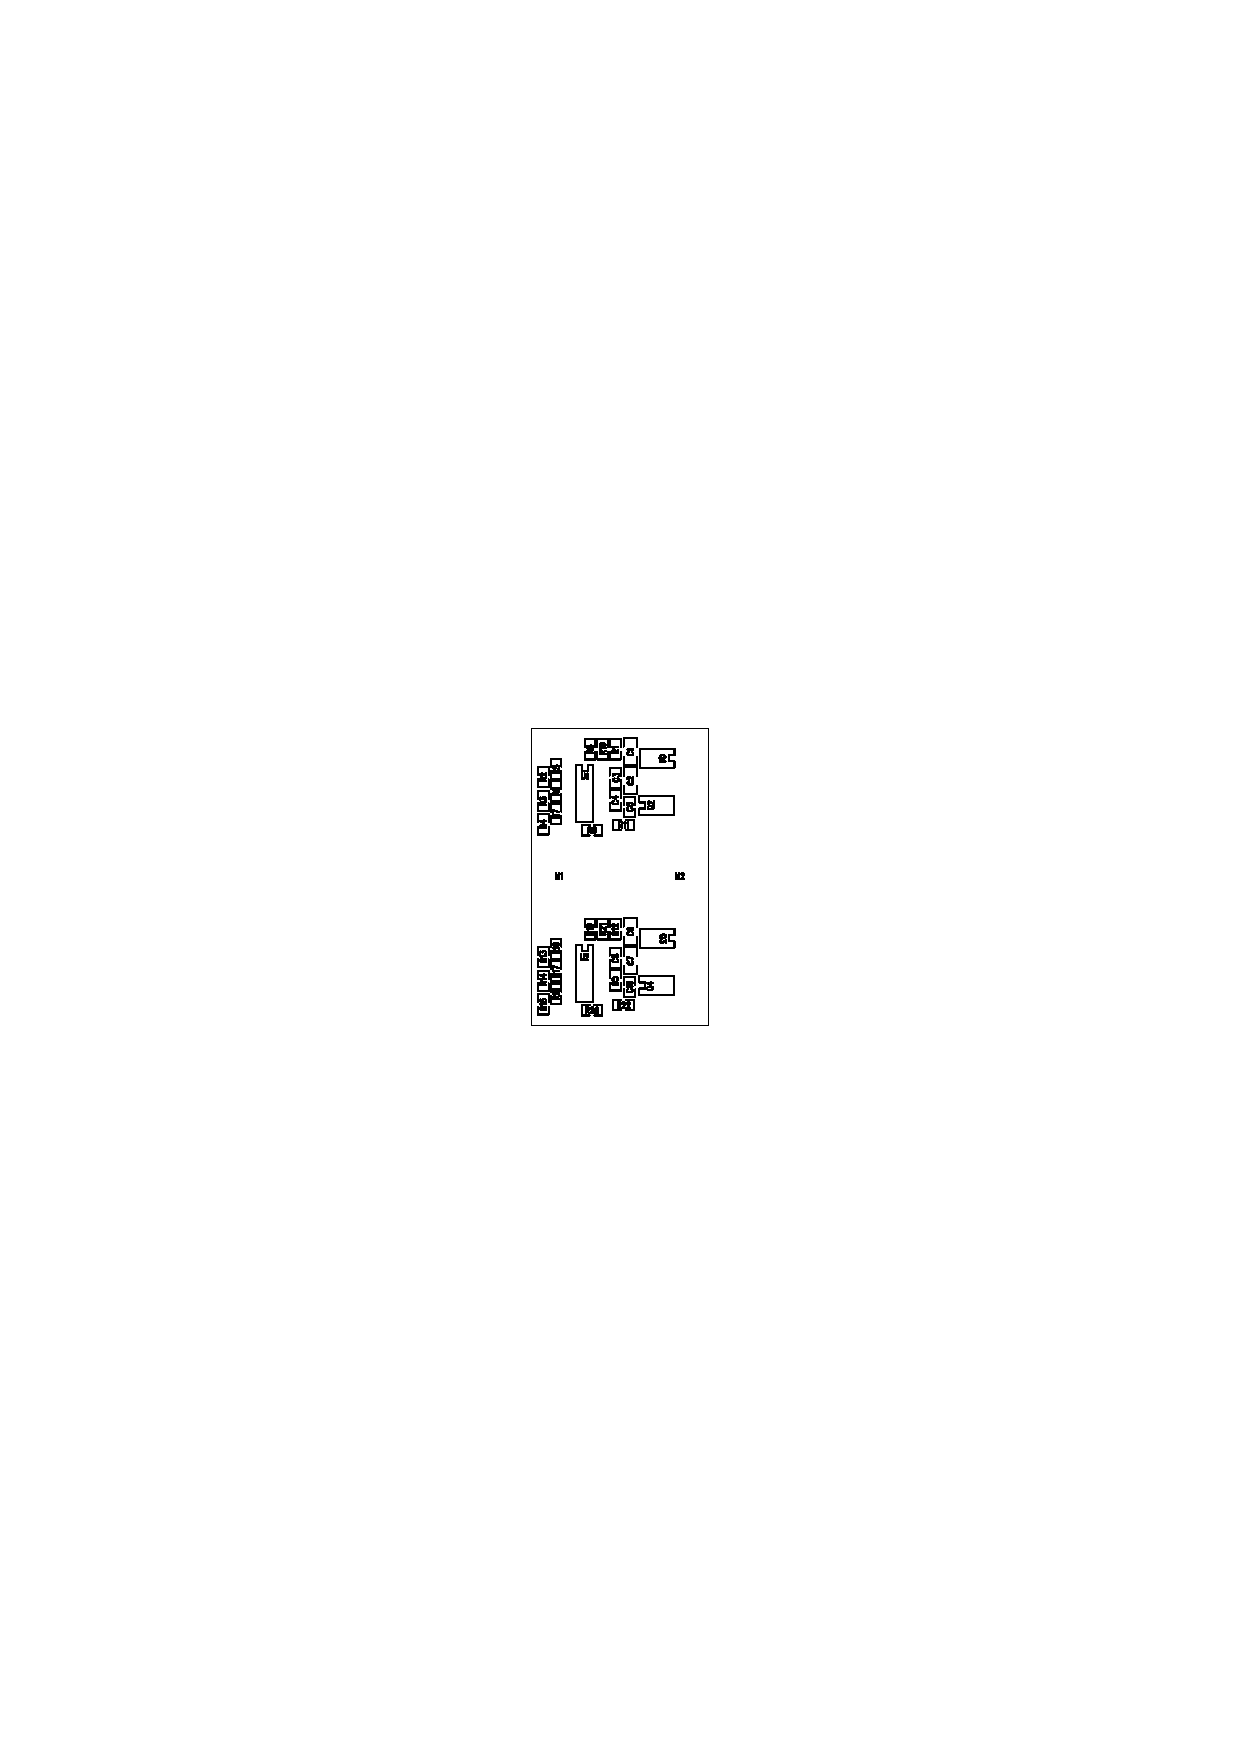
\includegraphics[trim = 8.0cm 9.5cm 8.0cm 9.5cm, clip, width=6cm]{../../CAM_DOC/O1.pdf}
  %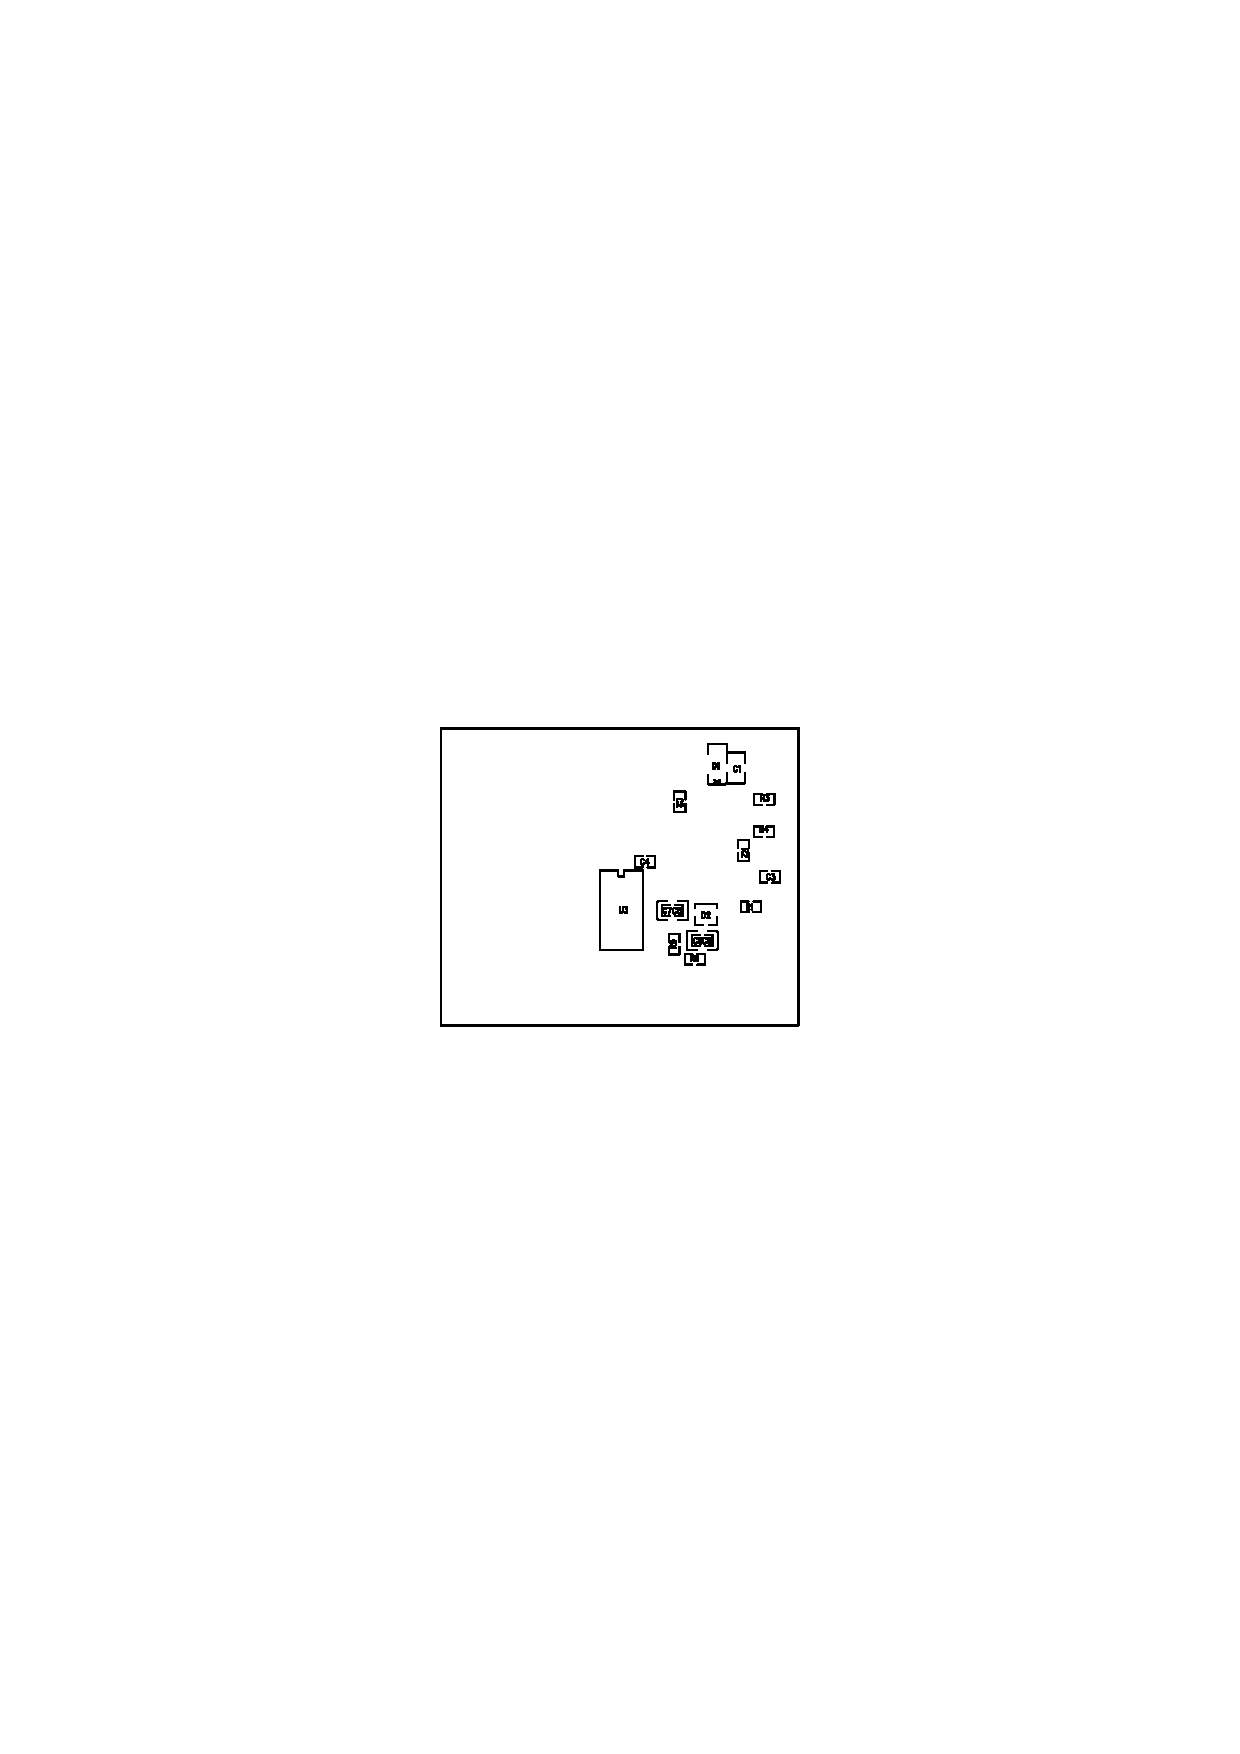
\includegraphics[trim = 8.0cm 9.5cm 8.0cm 9.5cm, clip, width=6cm]{../../CAM_DOC/O2.pdf}
  \caption{Osazovací plán horní a spodní strany plošného spoje}
  \label{fig:osazovaci_plan}
\end{figure}

\begin{savenotes}
\begin{table}[h!]
\begin{center}
\begin{tabular}{ |c|c|c|c| }
\hline 
Počet & Označení & Typ  & Pouzdro  \\ 
\hline 
10	&	C1,C3,C6,C7,C8,C9,C10,C11,C12,C13	&	100nF	&	C0805	\\
1	&	C2	&	20uF	&	ELYTC	\\
2	&	C4,C5	&	12pF	&	C0805	\\
1	&	C14	&	22uF	&	ELYTC	\\
1	&	D1	&	M4	&	SMA	\\
1	&	J1	&	USB\_B\_01	&	USB\_B\_01	\\
4	&	J2,J3,J13,J14	&	JUMP2X3	&	JUMP2X3	\\
2	&	J4,J8	&	JUMP2X4	&	JUMP2X4	\\
1	&	J5	&	JUMP2X8	&	JUMP2X8	\\
1	&	J6	&	JUMP2X6	&	JUMP2X6	\\
2	&	J9,J11	&	JUMP2X1	&	JUMP2X1	\\
2	&	J10,J12	&	JUMP2X2	&	JUMP2X2	\\
1	&	L1	&	MI0805K400R-10	&	R0805	\\
1	&	R1	&	100k	&	R0805	\\
2	&	R2,R3	&	2K2	&	R0805	\\
1	&	R4	&	10K	&	R0805	\\
1	&	R5	&	1K	&	R0805	\\
1	&	SW1	&	PUSH050x050	&	PUSH050x050	\\
1	&	U1	&	CY7C68013A	&	SSOP56\_300	\\
1	&	U2	&	LM1117MPX\_3V3	&	SOT223	\\
1	&	U3	&	TCM809	&	SOT23	\\
1	&	X1	&	24MHz	&	XTAL050	\\
\hline 
\end{tabular}
\end{center}
\caption{Seznam součástek osazovaných na desku plošného spoje.}
\label{seznam_soucastek_galvanic_isolation}
\end{table}
\end{savenotes}

\begin{thebibliography}{99}

\end{thebibliography}
\end{document}